
\documentclass[12pt, reqno]{amsart}
\usepackage{amsmath, amsthm, amscd, amsfonts, amssymb, graphicx, xcolor}
\usepackage{todonotes}
\usepackage[bookmarksnumbered, colorlinks, plainpages]{hyperref}
\usepackage{tikz}
\usepackage{tikz-3dplot} % Do rysowania w 3D
\usetikzlibrary{calc} % Potrzebne do obliczania punktow na odcinkach
\usepackage{tikz-3dplot}
\usetikzlibrary{patterns}

\textheight 22.5truecm \textwidth 14.5truecm
\setlength{\oddsidemargin}{0.35in}\setlength{\evensidemargin}{0.35in}

\setlength{\topmargin}{-.5cm}

\newtheorem{theorem}{Theorem}[section]
\newtheorem{lemma}[theorem]{Lemma}
\newtheorem{proposition}[theorem]{Proposition}
\newtheorem{corollary}[theorem]{Corollary}
\theoremstyle{definition}
\newtheorem{definition}[theorem]{Definition}
\newtheorem{example}[theorem]{Example}
\newtheorem{exercise}[theorem]{Exercise}
\newtheorem{conclusion}[theorem]{Conclusion}
\newtheorem{conjecture}[theorem]{Conjecture}
\newtheorem{criterion}[theorem]{Criterion}
\newtheorem{summary}[theorem]{Summary}
\newtheorem{axiom}[theorem]{Axiom}
\newtheorem{problem}[theorem]{Problem}
\theoremstyle{remark}
\newtheorem{remark}[theorem]{Remark}
\numberwithin{equation}{section}

\newcommand{\interior}[1]{%
  {\kern0pt#1}^{\mathrm{o}}%
}

\begin{document}
\setcounter{page}{1}

\color{darkgray}{
\noindent 
%{\small Geometry and Topology}\hfill %{\small ISSN: 2789-7206}\\
%{\small Vol 20 (2024) 1-3}\hfill  {\small https://doi.org/10.56947/amcs.v20.223}}

\centerline{}

\centerline{}

\newcommand{\pknote}[1]{\todo[inline, color=cyan]{PK:\ #1}}
\newcommand{\term}[1]{\emph{#1}}

\newcommand{\wwnote}[1]{\todo[inline, color=yellow]{WW:\ #1}}

%------------------------------------------------------------------------------

%Title of the paper
\title[Generalization of Ceva theorem]{Generalization of Ceva theorem}

%Author names and affiliations
\author[Wojciech Wdowski]{Wojciech Wdowski}

%\address{$^{1}$ Department of Mathematics, University of California, San Diego, USA.}
%\email{\textcolor[rgb]{0.00,0.00,0.84}{first@amcs.org}}




%\dedicatory{This paper is dedicated to Professor ABCD}

%\date{Received: xxxxxx; Revised: yyyyyy; Accepted: zzzzzz.
%\newline \indent $^{*}$ Corresponding author
%\newline \indent © The Author(s) 2025. This article is licensed under a Creative Commons Attribution-
%\newline \indent NonCommercial-NoDerivatives 4.0
%International License. To view a copy of the licence, visit 
%\newline \indent \url{https://creativecommons.org/licenses/by-nc-nd/4.0/}}


%Abstract, keywords, math subject classification
\begin{abstract}
In this paper, we present a novel generalization of the classical Ceva theorem to arbitrarily dimensional simplexes. Our approach allows cevians to have any dimension (smaller than the dimension of the base simplex). Consequently, our result unifies other generalizations of the Ceva theorem obtained in recent years.
% Wiekszośc stylow czasowpism oferuje wlasne polecenie do tworzenie 
% slow kluczowych I kodow MSC$
\noindent \\\textit{Keywords.} Geometry, simplex, Ceva's theorem 
\end{abstract} \maketitle
%\pknote{Prerobiłem abstrakt.}
%\wwnote{Done.}

\section{Introduction}

\subsection{Ceva's Theorem}\label{Ceva's theorem}
Ceva's Theorem---first proved by Yusuf al-Mu'taman ibn Hud, a king of~Zaragoza---is a fundamental result in the classical $2$-dimensional geometry. Although we firmly believe that it is well known to the readers, we nonetheless recall it here to make the whole exposition cleaner.

\begin{theorem}[Ceva's Theorem]
  Let $\Delta P_0P_1P_2$ be a triangle, and let points $Q_0,Q_1,Q_2$ lie on the edges opposite to vertices $P_0,P_1,P_2$, respectively \textup(see Figure~\ref{fig:trojkat_punkty_Q}\textup). Then, simplices $P_iQ_{i}$ \textup(for $i\in\{0,1,2\}$\textup) intersect nonempty if and only if the following formula holds
  \[
  \frac{P_0Q_1}{Q_1P_2}\frac{P_2Q_0}{Q_0P_1}\frac{P_1Q_2}{Q_2P_0}=1.
  \]
\end{theorem}

Recall that the segment $P_iQ_{i}$ is called a \term{cevian}, and point $Q_{i}$ is called \term{cevian's foot} (for $i\in\{0,1,2\}$).
\begin{figure}\label{fig:trojkat_punkty_Q}
  \centering
  \begin{tikzpicture}[scale=0.9]
  % Definiowanie wspolrzednych wierzcholkow trojkata P
  \coordinate (P0) at (0,0);
  \coordinate (P1) at (6,1);
  \coordinate (P2) at (1,3);
  

  % Opisywanie wierzcholkow trojkata
  \node[below left] at (P0) {$P_0$};
  \node[right] at (P1) {$P_1$};
  \node[above left] at (P2) {$P_2$};
  
  % Definiowanie punktow Q na przeciwleglych bokach
  % Q0 na boku P1P2 (np. w polowie, 0.5 to środek)
  \coordinate (Q0) at ($ (P1)!0.7!(P2) $);
  % Q1 na boku P0P2
  \coordinate (Q1) at ($ (P2)!0.3!(P0) $);
  % Q2 na boku P0P1
  \coordinate (Q2) at ($ (P0)!0.5!(P1) $);

  % Rysowanie i opisywanie punktow Q na czerwono
  \fill (Q0) circle (1pt) node[above] {$Q_0$};
  \fill (Q1) circle (1pt) node[left] {$Q_1$};
  \fill (Q2) circle (1pt) node[below] {$Q_2$};

  %rysowanie lini
  \draw (P0) -- (Q0);
  \draw (P1) -- (Q1);
  \draw (P2) -- (Q2);

  % Rysowanie trojkata P_0 P_1 P_2
  \draw[thick] (P0) -- (P1) -- (P2) -- cycle;

  \end{tikzpicture}
  \caption{Demonstration of Ceva's Theorem.}
\end{figure}
%\pknote{Wiekszość czasopism nie lubi rysunków w środku tekstu i opcji [h] w otoczeniach figure.}
%\wwnote{Not Done.}

This paper aims to extend the above result to simplices of arbitrary dimensions. Prior work on this topic has been conducted in \cite{Buba-Brzozowa, Prince, Samet, Witczynski}. In all four papers, the authors used an $n$-dimensional simplex as a (natural) generalization of a triangle. However, the notion of a cevian differs between the papers. Witczyński and Buba-Brzozowa (see \cite{Witczynski,Buba-Brzozowa}) use $(n-1)$-dimensional simplices to generalize the concept of a cevian. On the other hand, in Samet's paper \cite{Samet}, cevians are simply $1$-dimensional. These two interpretations exhaust the possibilities for defining cevians in three-dimensional space. However, in higher dimensions, there are other possibilities. For example, when the dimension equals~$4$, one may think of $2$-dimensional cevians and ask whether an analogous result holds.

Below, we present a result (see Theorem~\ref{Main!}) that generalizes the Ceva theorem to simplices of an arbitrary dimension $n\geq 2$ and cevians of dimension~$k$ for any $1 \leq k < n$. Our result encompasses and extends those of Witczyński, Buba-Brzozowa, and Samet. In fact, the above-mentioned theorems appear as border cases of our main result.

Similar results have already been obtained in \cite{Prince}, by means of algebraic geometry techniques. In contrast, the present work uses a much simpler method to obtain the same conclusions, while also provide a straightforward condition for every $k\in\{1,...,n\}$. 

For a complete understanding of this paper (besides a working knowledge of $n$-dimensional real space), we assume familiarity with the framework developed in \cite{Samet}.

\subsection{Simplices}\label{symplex}
Let $P_0P_1\dots P_n$ be points in a general position of an $n$-dimensional Euclidean space. We denote by $\mathbf{S} = \Delta P_0P_1\dotsc P_n$, the $n$-dimension simplex spanned by these points. The \term{interior} of the simplex $\mathbf{S}$, denoted~$\interior{\mathbf{S}}$, is the set of points of the form 
\[
\alpha_0P_0+\dotsb +\alpha_nP_n, 
\]
where $\sum^n_{k=0}\alpha_k=1$ and $\alpha_k>0$ for every~$k$.

Any subset of $k+1$ points from $\{P_0,P_1,\dots,P_n\}$ spans a $k$-dimensional \term{subsimplicial face} of~$\mathbf{S}$, which we refer to as a $k$-\term{face} (or simply \term{face}). In particular, when $k = n - 1$, the resulting $(n-1)$-face is called a \term{facet}. We denote by $\mathbf{S}_i$ the facet of~$\mathbf{S}$ opposite to the vertex~$P_i$, i.e., the facet that does not contain~$P_i$. %The collection of all faces of~$\mathbf{S}$ will be denoted by~$\mathcal{F}$.

\subsection{Construction of $k$-dimension cevians}\label{construction}
We begin by defining the notion of $k\mbox{-cevians}$. Assume that the simplex~$\mathbf{S}$ is fixed once and for all. Take a subset $U = \{u_1,\dotsc ,u_k\}$ of the set of indices $\{0,\dotsc ,n\}$, where $0\leq u_1<u_2<\dotsb <u_k\leq n$. Denote its completion by $U' = \{0,\dotsc ,n\}\setminus U$, and assume that $U'=\{v_1,\dotsc ,v_l\}$, where $0\leq v_1<v_2<\dotsb <v_{l}\leq n$ and $k+l=n+1$. Next, select a point $Q_{U'}$ in the interior of $\Delta P_{v_1}\dotsc P_{v_l}$. The simplex $\Delta Q_{U'}P_{u_1}\dotsc P_{u_k}$ will be called a \term{$k\mbox{-cevian}$} of $\mathbf{S}$. 

The point $Q_{U'}$ will be referred to as the \term{foot} of the $k$-cevian. In an $n\mbox{-dimensional}$ simplex, there are ${n+1 \choose k}$ possible choices for the set~$U$. Assume that for each such choice, we have selected a corresponding foot $Q_{U'}$. This way, we obtain a family of ${n+1 \choose k}$ $k\mbox{-cevians}$, which we denote by~$\mathfrak{R}$. 

Theremainder of the paper will be devoted to finding conditions on simplices that ensure that the family~$\mathfrak{R}$ has a nonempty intersection In what follows, the family~$\mathfrak{R}$ of $k\mbox{-cevians}$, like the simplex~$\mathbf{S}$, will be assumed to be fixed.

%$Such a problem has already been studied in \cite{Prince} 

\subsection{\texorpdfstring{$l$-Faces}{l-Faces}}
An essential role in the subsequent discussion will be played by the $l$-dimensional faces of~$\mathbf{S}$, where $k + l = n + 1$. Accordingly, we will study the relationship between the $k$-cevians and the $l$-faces.

Let $\mathbf{L}$ be an $l$-face of the form  
\[
\mathbf{L}=\Delta P_{j_0}\dotsc P_{j_l},
\]
where $J=\{j_0,\dotsc ,j_l\}\subset\{0,1,...,n\}$. Let $J' = \{ i_1, \dotsc, i_{k-1} \} = \{ 0, \dotsc, n \} \setminus J$ denote the complement of $J$.

Observe that each \emph{facet} of~$\mathbf{L}$---that is, each $(l-1)$-dimensional face of $\mathbf{L}$---contains exactly one foot of a $k$-cevian from the family~$\mathfrak{R}$. Specifically, for each $t\in J$, the interior of the facet ${\mathbf{L}_t}$, spanned by $\{ P_j: j\in J, j\neq t\}$, contains the foot~$Q_{J\backslash\{t\}}$ of a $k$-cevian
\begin{equation} \label{form}
C_t = \Delta Q_{J\backslash\{t\}} P_t P_{i_1} \dotsc P_{i_{k-1}}.
\end{equation}
Moreover, every $k$-cevian whose foot lies in a facet of~$\mathbf{L}$ is of the form \eqref{form}. Thus, the subfamily of $\mathfrak{R}$ consisting of $k$-cevians whose feet lie in~$\mathbf{L}$ has precisely $l+1$ elements. We denote this subfamily by~$\mathfrak{R}_\mathbf{L}$.

%\pknote{Tu wciaz jest problem z notacja. Raz mamy $C_{U'}$, gdzie $U'$ jest podzbiorem, a tutaj zas $C_t$, gdzie $t$ jest pojedynczym indeksem.}
%\wwnote{Done.}

Throughout the rest of the paper, while analyzing the cevian feet within a given $l$-face, we shall adopt the notation $Q_{[t]}$ in place of $Q_{J\backslash\{t\}}$.%\textit{ To prevent any confusion for the reader, superscript be used when indexing by numbers, and subscripts when indexing by sets.}

%\wwnote{Widze dwa rozwiazania: Zamiana wszystkich $Q_{[t]}$ na $Q_{J\backslash\{t\}}$ albo dopisany tu paragraf (+ewentualna zmiana indeksu z dolnego na gorny w przypadku gdy indeksujemy pojedyńczym indeksem). Drugie rozwiazanie wydaje mi sie byc bardziej czytelnym, bo nie wymaga zawsze wypisywania postaci $J$.}
%\pknote{Myśle, że tak może być. Ewentualnie zamiast indeksu górnego, może $Q_{[t]}$, bo faktycznie $Q_{J\setminus \{t\}}$ jest nieco rozwlekłe.}
%\wwnote{Not done.}

\subsection{Induced cevians}
Given an $l$-face~$\mathbf{L}$ of~$\mathbf{S}$ and a $k$-cevian $C_t\in\mathfrak{R}_\mathbf{L}$ with foot~$Q_{[t]}$ in the interior of~$\mathbf{L}$ we define the \term{induced cevian}~$c_t$ in~$\mathbf{L}$ as the intersection 
\[
c_t = C_t\cap\mathbf{L} = \Delta Q_{[t]}P_t.
\]
In this way, we obtain a family of $1$-cevians in~$\mathbf{L}$, defined as in~\cite{Samet}, which we denote by $\mathfrak{r}_\mathbf{L}$. 

Before proceeding further, we present two examples that illustrate the notions introduced above and place them in the proper context with respect to prior work.
  
\begin{example}[Case $n=3\text{ and }k=2$]
Let $\mathbf{S} = \Delta P_0P_1P_2P_3$ be a simplex. Construct a $2$-cevian in~$\mathbf{S}$. To this end take a set $U=\{2,3\}$ (so $U'=\{0,1\}$), and select a point $Q_{U'}\in\interior{\Delta P_0P_1}$. Then the simplex $C = \Delta Q_{U'}P_2P_3$ is a $2\mbox{-cevian}$ (see Figure~\ref{n=3,k=2}).

Since $k=2$, we have that $l=2$. Therefore, $\mathbf{L}=\Delta P_0P_1P_3$ is a $2\mbox{-face}$ of $\mathbf{S}$. Then $Q_{U'}=Q_{[3]}$,
\[
C=C_3=\Delta Q_{[3]}P_3P_2
\]
and the induced cevian~$c_3$ in~$\mathbf{L}$ has the form $c_3=\Delta Q_{[3]}P_3$. It is a line segment, and so a cevian in the most classical sense.

Moreover, as $k=n-1$, the $2$-cevian~$C$ is a cevian in the sense of \cite{Witczynski} and \cite{Buba-Brzozowa}.
\end{example}
%\pknote{Nadal mi sie tu coś nie zgadza w indeksacji. Skoro jesteśmy na ścianie $\Delta P_0P_1P_3$, to indukowany cevian powinien mieć postać $\Delta Q_{U'}P_3$, a nie $P_2$.}
%\wwnote{Done.}

\begin{figure}  
\centering  
\tdplotsetmaincoords{70}{110} % Setting the perspective (theta, phi angles)  
\begin{tikzpicture}[tdplot_main_coords, scale=4]  

% Vertex definitions  
\coordinate (P0) at (-0.5,0.2,0);  
\coordinate (P1) at (1.2,0,0);  
\coordinate (P2) at (0.5,1.2,0);  
\coordinate (P3) at (0.5,0.5,1);  

% Drawing the tetrahedron's edges  
% Visible edges  
\draw[thick] (P0) -- (P1);  
\draw[thick] (P0) -- (P2);  
\draw[thick] (P1) -- (P2);  
\draw[thick] (P0) -- (P3);  
\draw[thick] (P1) -- (P3);  
\draw[thick] (P2) -- (P3);  

% Filling the triangle P0P1P3 with dots  
\filldraw[opacity=0.5, thick, pattern=dots] (P0) -- (P1) -- (P3) -- cycle;  

% Vertex labels  
\node at (P0) [above right] {$P_0$};  
\node at (P1) [below] {$P_1$};  
\node at (P2) [right] {$P_2$};  
\node at (P3) [above] {$P_3$};  

% Point Q_U' on the edge P0P1  
% We use the "pos" function to place the point inside the edge  
% pos=0.5 means the midpoint, you can change this value  
\path (P0) -- (P1) coordinate[pos=0.4] (QUprime);  
\node[below right] at (QUprime) {$Q_{U'}$}; % Point label  


% NEW ELEMENTS:  
% Blue lines from Q_U' to P2 and P3  
\draw[thick] (QUprime) -- (P2);  
\draw[thick] (QUprime) -- (P3);  

% Filling the triangle P2P3Q_U' with vertical lines  
\filldraw[opacity=0.5, thick, pattern=vertical lines] (P2) -- (P3) -- (QUprime) -- cycle;  
\fill (QUprime) circle (0.5pt); % Draws a red circle  
\end{tikzpicture}  
\caption{\label{n=3,k=2}Case $n=3, k=2$ with the $2\mbox{-cevian } C$ is dashed and the $2\mbox{-face } \mathbf{L}$ is dotted.}  
\end{figure}


%\pknote{Kolorowe rysunki bywaja problemem w publikacjach matematycznych.}
%\wwnote{Not Done.}

\begin{example}[Case $n=4$, $k=2$]
Now consider a $4$-dimensional simplex $\mathbf{S} = \Delta P_0P_1P_2P_3P_4$. We again construct a $2$-cevian in $\mathbf{S}$. Let $U=\{2,4\}$, so its complement is $U' = \{0,1,3\}$. Choose a point $Q_{U'}$ in the interior of the subsimplex $\Delta P_0P_1P_3$. Then the simplex $C=\Delta Q_{U'}P_2P_4$ (see Figure~\ref{n=4,k=2}) is a $2$-cevian in~$\mathbf{S}$.

In this case, $k=2$ and $l=3$, so $\mathbf{L}=\Delta P_0P_1P_2P_3$ is a $3$-dimensional face of~$\mathbf{S}$. Then $Q_{U'}=Q_{[2]}$,
\[
    C=C_2=\Delta Q_{[2]}P_2P_4
\]
and the induced cevian~$c_2$ is of the form  
\[
c_2 = \Delta Q_{[2]} P_2. %dopisac na jaki L symplex jest indukowane
\]

It should be emphasized that the cevian $C$ is neither a line segment nor a simplex of codimension one. To the best of the author's knowledge, such cases have not been treated in previous literature.
\end{example}

\begin{figure}
\centering
\tdplotsetmaincoords{70}{110} % Ustawienie perspektywy (kat theta, kat phi)
  \begin{tikzpicture}[tdplot_main_coords, scale=4]
    
      
      % Definicja wierzcholkow
      \coordinate (P0) at (-0.5,0.2,0);
      \coordinate (P1) at (1.2,0,0);
      \coordinate (P2) at (0.5,1.2,0);
      \coordinate (P3) at (0.5,0.5,1);
    
      % NOWY PUNKT: P4
      % Pozycja "lewo gora od czworościanu" wymaga eksperymentowania.
      % Dostosuj te wspolrzedne, jeśli chcesz innej pozycji.
      \coordinate (P4) at (-1, 1, 0.5);
      \node at (P4) [above left] {$P_4$};

     % NOWA KROPKA: Mala czarna kropka w miejscu P4
        \fill[black] (P4) circle (0.4pt); % Rysuje male czarne kolko
        
      % Rysowanie krawedzi czworościanu
      \draw[thick] (P0) -- (P1);
      \draw[thick] (P0) -- (P2);
      \draw[thick] (P1) -- (P2);
      \draw[thick] (P0) -- (P3);
      \draw[thick] (P1) -- (P3);
      \draw[thick] (P2) -- (P3);
    
      % Etykiety wierzcholkow
      \node at (P0) [above right] {$P_0$};
      \node at (P1) [below] {$P_1$};
      \node at (P2) [right] {$P_2$};
      \node at (P3) [above] {$P_3$};

      % NOWE LINIE:
    % Linie przerywane od P4 do P0, P2, P3
    \draw[dashed, thick] (P4) -- (P0);
    \draw[dashed, thick] (P4) -- (P2);
    \draw[dashed, thick] (P4) -- (P3);

    % ZMIANY: Wypelnienie czworościanu P0P1P2P3 na zolto - KROPKI
    % Rysowanie i wypelnianie ścian, zaczynajac od tych "niewidocznych"
    % Uzyj opacity, zeby widziec wnetrze
    \filldraw[opacity=0.2, thick, pattern=dots] (P0) -- (P1) -- (P2) -- cycle; % Podstawa
    \filldraw[opacity=0.2, thick, pattern=dots] (P0) -- (P1) -- (P3) -- cycle; % Jedna ze ścian bocznych
    \filldraw[opacity=0.2, thick, pattern=dots] (P0) -- (P2) -- (P3) -- cycle; % Kolejna ściana boczna
    \filldraw[opacity=0.2, thick, pattern=dots] (P1) -- (P2) -- (P3) -- cycle; % Ostatnia ściana boczna
    
    % Krzywa linia przerywana od P4 do P1
    \draw[dashed, thick] (P4) .. controls (-0.5, 2, 0.4)  and (0.5, 1.5, -0.6) .. (P1);

    % NOWY PUNKT: Q_U' wewnatrz trojkata P0P1P3
    \coordinate (QUprime) at ($(P0)!0.33!(P1)!0.3!(P3)$); 
    \fill (QUprime) circle (0.5pt); % Mala czerwona kropka
    \node[below] at (QUprime) {$Q_{U'}$}; % Etykieta punktu

    % ZMIANY: Niebieskie linie laczace P2, P4 i Q_U' - KRESKI
    \draw[black, thick] (P2) -- (P4) -- (QUprime) -- (P2);
    \filldraw[black, opacity=0.5, thick, pattern=vertical lines] (P2) -- (P4) -- (QUprime) -- cycle; 

  \end{tikzpicture}
  \caption{\label{n=4,k=2} Visualization for Case $n=4, k=2$. The $2\mbox{-cevian } C$ is dashed, and the $3\mbox{-face } \mathbf{L}$ is dotted.} 
\end{figure}

\subsection{Multipedes} 
%Finally, we need to recall the notion of a \term{multipede} and \term{induced multipede}, introduced originally by Samet in~\cite{Samet}. A set of point $\{A_{\mathbf{F}}\}_{\mathbf{F}\in \mathcal{F}}$ is called a \term{multipede}, if every point $A_\mathbf{F}$ is in the interior of the face $\mathbf{F}$.
%
%\pknote{$\mathcal{F}$ to rozdzina wszystkich scian CALEGO kompleksu~$\mathbf{S}$. Czy tu na pewno chcemy miec WSZYSTKIE sciany (=caly kompleks)? A nie przypadkiem wszystkie sciany JAKIEJSC sciany?}
%\wwnote{Tak, to powinno byc dla kompleksu pewnej sciany, ten problem sie rozwiazuje przez jedno z dzialan wymienionych w kolejnej notatce.}
%
%We say that a point $A_\mathbf{S}$ induces a multipede in a simplex $\mathbf{S}$ if points $A_\mathbf{S},A_{\mathbf{S}_i},P_i$ are in general position\todo{Niezdefiniowane obiekty $A_{\mathbf{S}_i}$, $P_i$}. Moreover, for every $1\mbox{-face}$ $\mathbf{F}\in\mathcal{F}$ (where $t> 1$) points $A_\mathbf{F},A_{\mathbf{F}_i},P_i$ are in general position. Samet proved that each point in the interior of a given simplex induces exactly one multipede.
%
%\pknote{Ta definicje multipede to trzeba by jeszcze wygladzic.}
%\wwnote{Punkty $P_i$ to wierzcholek rozpinajacy symplex $\mathbf{S}$, $\mathbf{S}_i$ jest zdefioniowane w rozdziale \eqref{symplex}, zatem $A_{\mathbf{S}_i}$ jest punktem z multipede lezacym w wnetrzu $\mathbf{S}_i$. Analogicznie, z \eqref{symplex} mamy $\mathbf{F}_i$ to facet $\mathbf{F}$ itd. 
%Natomiast rzeczywiscie jest tu problem, bo w rodziale \eqref{construction} ustalamy $\mathbf{S}$ raz na zawsze, a chcemy aby definiowac multipede w dowolnym sympleksie. Aby temu zarazic mozna przesunac ten rozdzial przed \eqref{construction}. Ewentualnie widze takie rozwiazanie:}
%\pknote{Zmieniłem $\mathbf{M}$ na $\mathbf{T}$ (wydaje sie lepsze, skoro sympleks to $\mathbf{S}$). Należałoby jeszcze wyjaśnić jak sie ma $P_i$ w kontekście $\mathbf{T}$, skoro teraz jest to ``any simplex''}
%\wwnote{Not Done.}
Finally, we recall the notion of a \term{multipede} and an \term{induced multipede}, introduced originally by Samet in~\cite{Samet}. Let~$\mathbf{T}$ be any $m~\mbox{- dimesional}$ simplex spanned by points from $\{P_0,P_1,...,P_m\}$ (in applications, it will be just a face of~$\mathbf{S}$). Denote by~$\mathcal{F}$ the collection of all faces of~$\mathbf{T}$. A set of points $\{A_{\mathbf{F}}\}_{\mathbf{F}\in \mathcal{F}}$ is called a \term{multipede} if every point $A_\mathbf{F}$ lies in the interior of the corresponding face~$\mathbf{F}$.

We say that a point $A_\mathbf{T}$ \term{induces} a multipede in a simplex~$\mathbf{T}$ if points $A_\mathbf{T}, A_{\mathbf{T}_i}, P_i$ are collinear. Moreover, for every $1\mbox{-face}$ $\mathbf{F}\in\mathcal{F}$ (where $t> 1$) points $A_\mathbf{F}, A_{\mathbf{F}_i}, P_i$ are collinear. Samet proved that each point in the interior of a given simplex induces exactly one multipede. 
%\wwnote{Jesli ta forma jest jasna, to moglbym tez zmienic wszedzie w \eqref{symplex} wszystkie $\mathbf{S}$ na $\mathbf{M}$ by odroznic definicje dla dowolnego sympleksu i dla tego wyroznionego $\mathbf{S}$.}

%Let $f$ be a function that maps
%\begin{enumerate}
%\item each point $A$ from the interior of $\mathbf{S}$ to a multipede induced by $A$ in $\mathbf{S}$.
%\item each point $A$ from the interior of a $t\mbox{-face}$ $\mathbf{F}$ (for $t>1$) to a multipede induced by $A$ in $\mathbf{F}$.
%\item each point $A$ from a $1\mbox{-face}$ $\mathbf{F}$ to set $\{A\}$. 
%\end{enumerate}
%There is a natural way to define a partial order for such points. Let $A,B$ be points from the domain of $f$, then $$A\preceq B \iff f(A)\subset f(B).$$

%\wwnote{
%Cala idea funkcji opiera sie na "lemacie": \textit{Samet proved that each point in the interior of a given simplex induces exactly one multipede.}
%Ad 2. W warunek (2) wkradla sie literowka, powinna tam byc $t$-face, juz to poprawilem. 

%Dziedzina funkcji $f$. Pierwotnie z uwagi na powyzsze lemat Sameta dziecina funckcji mialbyc caly sympleks bez wierzcholkow. (Lemat ten odnośic sie do wnetrza symplekow). Natomiast znalalem teraz sposob by dziedzia byl caly symplexm. To czysta formalnośc co zrobimy z wierzcholkami.

%Ad. 3. i 1. Opisywany przez Pana porzadek jest zadany przez inkluzje, oczywiscie mozna by pracowac juz z nim w tej formie, natomiast prościej jest pracowac na punktach (generatorach multipede) niz na multipede. Funkcja $f$ jest bijekcja mniedzy zbioramy tych obiektami i przenosi ona nam porzadek z multipede na punkty indukujace multipede.

%Ad. 4. Caly material "miedzy dowodem pierwsze i drugiej implikacji" znaczaco sie uprosil.}

%\pknote{Poniżej proponuje troche inne sfromułowanie definicji. IMHO bardziej czytelne}
%\wwnote{not Done.}
Let $\mathcal{M} = \{A_\mathbf{F}\}_{\mathbf{F}\in \mathcal{F}}$ be a multipede of~$\mathbf{T}$ induced by some point~$Q$. Fix a face~$\mathbf{F}\in \mathcal{F}$ of~$\mathbf{T}$ and let $P := A_\mathbf{F}$ be a point of the multipede~$\mathcal{M}$ in the interior of~$\mathbf{F}$. Then the multipede~$\mathcal{N}$ of~$\mathbf{F}$ induced by~$P$ is a subset of~$\mathcal{M}$. This inclusion let us define a relation $\preceq$ on the set of points of~$\mathbf{T}$. We say that $P\preceq Q$ if $P$ is one of the points of the multipede induced by~$Q$ (i.e., if the multipede induced by~$P$ is a subset of the multipede induced by~$Q$). This relation is not well-defined on the vertices of~$\mathbf{T}$. To remedy this, for any vertex~$P_i$ and a point~$Q$ in the interior of any face containing~$P_i$, we set $P_i\preceq Q$.
  
\section{Main results}

\begin{theorem}\label{main}
  Let $\mathfrak{R}$ be family of $k\mbox{-cevians}$ in $\mathbf{S}$.
  The following conditions are equivalent:
  \begin{enumerate}
  \item \label{1} $\underset{X\in\interior{S}}{\exists}X\in\bigcap\mathfrak{R}$ 
  \item \label{2} For every $l\mbox{-face}$ $\mathbf{L}$ we have $\bigcap\mathfrak{r}_\mathbf{L}\neq\emptyset$.
  \end{enumerate}
\end{theorem}

The proof of this theorem must be preceded by a lemma.

\begin{lemma}
Fix an $l$-face $\mathbf{L}$ and let $Q_{[i]}$ and $Q_{[j]}$ be feet of $k$-cevians lying in the interiors of the facets $\mathbf{L}_i$ and $\mathbf{L}_j$, respectively. Further, let $A$ and $B$ be points such that $A\preceq Q_{[i]}$, $B\preceq Q_{[j]}$ and $A,B\in\interior{\mathbf{F}}\subset\mathbf{L}$. Then condition~\eqref{2} of Theorem~\ref{main} implies that $A=B$.
\end{lemma}

\begin{proof}
 Let $X\in\bigcap\mathfrak{r}_\mathbf{L}$ then $Q_{[i]}\preceq X$ and $Q_{[j]}\preceq X$ so $A\preceq X$ and $B\preceq X$ since $A$ and $B$ are both in $\interior{\mathbf{F}}$, by \cite[Proposition~1]{Samet} it follows that $A=B$.
\end{proof}

%\pknote{Kilka problemów z tym lematem i jego dowodem (uczciwie to ja mogłem cześć wprowadzić "prostujac" jezyk).\\
%- $\mathfrak{r}_\mathbf{L}$ to rodzina cevianów, a nie punktów. zapis $X\in\mathfrak{r}_\mathbf{L}$ nie ma zatem sensu;\\
%- $\mathfrak{r}_\mathbf{L}$, w przeciwieństwie do np. $\mathbf{S}$ nie było ustalone, trzeba je albo ustalić w poprzedniej cześci artykułu, albo w wypowiedzi lematu;%\\
%- w wypowiedzi lematu pojawia sie $\interior{\mathbf{F}}$, należałoby doprecyzować jak sie ma $\mathbf{F}$ do $\mathbf{L}$;
%- domyślam sie, że ``it follows that $A=B$'' opiera sie o Sameta (że odpowiednie punkty indukowane różnymi ścieżkami sa dla wielonoga i tak jednozanczne), ale należałoby ten argument explicite podać.}
%\wwnote{Not Done. Podlinkować arugemnt od semeta.}



%\begin{remark}\label{important}
 %If condition~\eqref{2} holds, then each $t\mbox{-face}$ (where $1\leq t\leq l-1$) has exactly one point in its interior, which is generated by all $k\mbox{-Cevians}$ feet.
%\end{remark}
\begin{remark}\label{important}
 Let $W$ be the set of all points generated by all $k\mbox{-cevians}$ feet. If condition~\eqref{2} holds, then for each $t\mbox{-face}$ (where $1\leq t\leq l-1$) $\mathbf{T}$ we get
 \[
    |W\cup \interior{\mathbf{T}}|=1
 \]
\end{remark}
%\pknote{To nie tak, że każda ściana ma jedno-elementowe wnetrze (to byłoby niemożliwe w topologii euklidesowej), tylko zawiera pojedynczy punkt z określonego wielonoga. Należałoby to tutaj doprecyzować.}
%\wwnote{Done.}

\begin{remark}\label{important2}
  Condition~\eqref{2} is equivalent to the following one
\begin{itemize}
\item For every $l$-dimensional face $L$, there exists a point~$X$ such that $$Q_{[t]}\preceq X$$ for all $t$, where $Q_{[t]}$ is foot of a $k\mbox{-cevian}$ $C_t\in \mathfrak{R}_\mathbf{L}$ (i.e., $Q_{[t]}$ is a foot of induced cevian $c_t\in \mathfrak{r}_\mathbf{L}$).
\end{itemize}
\end{remark}

We are now in a position to prove the main theorem.

\begin{proof}[Proof of Theorem~\ref{main}]
Suppose that condition~\eqref{1} holds. Without loss of generality, we may assume that~$\mathbf{L}$ has the form $\mathbf{L}=\Delta P_0...P_l$. Then, any cevian~$C_t$ in $\mathfrak{R}_\mathbf{L}$ can be expressed as 
\[
C_t=\Delta Q_{[t]}P_t P_{l+1}...P_{n},
\]
where $t\in \{0,...,l\}$. Take a point $X\in \bigcap\mathfrak{R}$, then $X\in \interior{\mathbf{S}}$ and so $X$ is convex combination of the points $P_0P_1...P_n$ with weights $\alpha_0,...,\alpha_n$, where $\alpha_m>0$ and $\sum_{m=1}^n a_m = 1$. Consequently, 
\[
X=\alpha_0 P_0+\alpha_1P_1+ \dotsb +\alpha_{n}P_n.
\]
On the other hand, $X\in C_t$ and $X\in C_s$ for $s,t\in\{0,...,l\}$. It follows that $X$ has the form
\begin{equation}\label{!1}
\begin{cases}
  X &= \beta_1Q_{[t]}+\beta_2P_t+\alpha_{l+1}P_{l+1}+ \dotsb +\alpha_{n}P_n\\
  X &= \gamma_1Q_{[s]}+\gamma_2P_s+\alpha_{l+1}P_{l+1}+ \dotsb +\alpha_{n}P_n.
\end{cases}
\end{equation}
  %$$x=\beta_1Q_{[t]}+\beta_2P_t+\alpha_{l+1}P_{l+1}+...+\alpha_{n}P_n$$
  %$$ x=\gamma_1Q_{[s]}+\gamma_2P_s+\alpha_{l+1}P_{l+1}+...+\alpha_{n}P_n.$$
Notice that the uniqueness of barycentric coordinates implies that all the coefficients that correspond to the points $P_{l+1}, \dotsc, P_{n}$ are the same in all three representations. 

Set $\hat X:=\frac{\beta_1}{\beta_1+\beta_2}Q_{[t]}+\frac{\beta_2}{\beta_1+\beta_2}P_t$. It is clear that $\hat X\in\Delta Q_{[t]}P_t$. We claim that $\hat X\in \Delta Q_{[s]}P_s$. %By cutting tail property we have $$\beta_1\vec{0Q_{[t]}}+\beta_2\vec{0P_t}=\gamma_1\vec{0Q_{[s]}}+\gamma_2\vec{0P_s}$$
Denote $K := \sum_{m=l+1}^n\alpha_mP_m$. Then \eqref{!1} yields
\[
  (\beta_1+\beta_2)\cdot\Bigl(\frac{\beta_1}{\beta_1+\beta_2}Q_{[t]}+\frac{\beta_2}{\beta_1+\beta_2}P_t\Bigr)+K
  =
  (\gamma_1+\gamma_2)\cdot \Bigl(\frac{\gamma_1}{\gamma_1+\gamma_2} Q_{[s]}+\frac{\gamma_2}{\gamma_1+\gamma_2}P_s\Bigr)+K.
\]
Now, $\beta_1+\beta_2=1-\alpha_{l+1}+ \dotsb +\alpha_{n}=\gamma_1+\gamma_2$ and so we have
\[
  (\beta_1+\beta_2)(\frac{\beta_1}{\beta_1+\beta_2}Q_{[t]}+\frac{\beta_2}{\beta_1+\beta_2}P_t)+K
  =({\beta_1+\beta_2})(\frac{\gamma_1}{\gamma_1+\gamma_2} Q_{[s]}+\frac{\gamma_2}{\gamma_1+\gamma_2}P_s)+K.
\]
This implies that
\[
  \hat X=\frac{\gamma_1}{\gamma_1+\gamma_2} Q_{[s]}+\frac{\gamma_2}{\gamma_1+\gamma_2}P_s.
\]
Consequently, $\hat{X}\in\Delta Q_{[s]}P_s$ as claimed. This proves that $\bigcap\mathfrak{r}_\mathbf{L}$ is not empty.

Conversely, assume that condition~\eqref{2} holds. If the dimension~$n$ of the simplex~$\mathbf{S}$ is either $2$ or $3$, then the implication $\eqref{2} \Rightarrow \eqref{1}$ is already known. Specifically, it follows from the classical Ceva’s theorem when $n = 2$, and from its generalizations in the case $n = 3$: either from \cite{Buba-Brzozowa, Witczynski} when $k = 2$, or from \cite{Samet} when $k = 1$. Therefore ,we may assume that $n \geq 4$. The proof proceeds by induction on the dimension $k$ of the cevians involved. The base case $k = n-1$ is established in \cite{Buba-Brzozowa}. Assuming the result holds for some $1 < k < n$, we aim to show that it also holds for $k - 1$.
  
Let $\mathfrak{R}^{k-1}$ be a family of $(k-1)$-cevians in $\mathbf{S}$ satisfying~\eqref{2}. We shall construct a family~$\mathfrak{R}$ consisting of $k\mbox{-cevians}$. By Remark~\ref{important} there are precisely ${n+1 \choose l}={n+1 \choose n+1-k}={n+1 \choose k}$ points generated by feet of $(k-1)\mbox{-cevians}$ in the interiors of each $(l-1)\mbox{-face}$.  Let $Q_{U'}$ lie in the interior of an $(l-1)\mbox{-face}$ $\mathbf{F}$ of the form 
\[
\mathbf{F}=\Delta P_{v_1}...P_{v_l},
\]
where $0\leq v_1<v_2< \dotsb <v_{l}\leq n$. Take $U= \{0,\dotsc ,n\}\setminus\{v_1,v_2,\dotsc, v_{l}\}$, say $U=\{u_{1},...,u_k\}$ and $0\leq u_1<u_2< \dotsb <u_{k}\leq n$. Then the simplex 
\[
C=\Delta Q_{U'}P_{u_1}...P_{u_k}
\]
is a $k\mbox{-cevian}$. Repeating this procedure for different points $Q_{U'}$ we obtain a family~$\mathfrak{R}$ consisting of  $n+1 \choose k$ $k\mbox{-cevians}$. It follows from Remark~\ref{important2}, that $\mathfrak{R}$, satisfies~\eqref{2}. Hence, by the inductive hypothesis, there exists a point $X\in \mathfrak{R}$. 
  
To conclude the proof, we need to show $X$ sits in~$\mathfrak{R}^{k-1}$. To this end, take a  $(k-1)$-cevian $\hat{C}=\Delta\hat{Q}P_{i_1}\dotsc P_{i_{k-1}}$, where $\hat{Q}\in\interior{\mathbf{L}}$ is a foot of $\hat{C}$ and $\mathbf{L}={\Delta P_{j_0}\dotsc P_{j_l}}$. Every point in $\hat{C}$ can be expressed as a convex combination 
\[
\hat \omega \hat Q+\omega_1P_{j_1}+ \dotsb +\omega_{k-1}P_{k-1}.
\]
We claim that the point~$X$ also has this form. Since $X\in\interior{\mathbf{S}}$, it~follows that it can be expressed as
\[
X=\alpha_0P_0+\alpha_1P_1+ \dotsb +\alpha_nP_n,
\]
where $\alpha_m>0$ and $\sum^n_{m=0}a_m=1$. Moreover, the fact that $X$ sits in $\mathfrak{R}$ implies that $X\in C_t$, where 
\[
C_t=Q_{[t]}P_tP_{i_1}\dotsc P_{i_{k-1}},
\]
for some $Q_{[t]}\in\mathbf{L}_t$ and $t\in\{j_0,\dotsc ,j_l\}$. Consequently, we have 
\[
X=\beta_1Q_{[t]}+\beta_2P_t+\alpha_{i_1}P_{i_{1}}+\dotsb +\alpha_{i_{k-1}}P_{i_{k-1}}.
\]
Thus, $\hat{Q}=\frac{\beta_1}{\beta_1+\beta_2} Q_{[t]}+\frac{\beta_2}{\beta_1+\beta_2}P_t$ and so putting $\hat \omega=\beta_1+\beta_2$ and $\omega_m=\alpha_{i_{m}}$, we obtain $X\in \hat{C}$. This concludes the proof.
\end{proof}

The preceding result can now be reformulated in a manner analogous to the classical Ceva’s theorem.

\begin{theorem} \label{Main!}
Let $\mathfrak{R}$ be a family of $k\mbox{-cevians}$ in $\mathbf{S}$. The following conditions are equivalent:
  \begin{enumerate}
  \item \label{1!} The family $\mathfrak{R}$ intersects nonempty.
  \item \label{2!} For every $l\mbox{-face}$ $\mathbf{L}$ and every uniform or mixed fan $\{(F_z,L_z,M_z)| z\in\mathbb{Z}/m\mathbb{Z}\}$ one has
  $$\prod_{z\in\mathbb{Z}/m\mathbb{Z}} \frac{\mbox{Vol}(L_z)} {\mbox{Vol}(M_z)}=1$$
  \end{enumerate}
\end{theorem}

%\pknote{Ostatni wzór nie ma sensu. Rozumiem, że miało być $=1$.}
%\wwnote{Done.}
  
\begin{proof}
The second conditions of Theorems~\ref{main} and~\ref{Main!} are equivalent, as shown in \cite{Samet}.
\end{proof}

Finally, let us point out that the results in \cite{Buba-Brzozowa, Witczynski, Samet} as well as the classical Ceva's theorem are special cases of Theorem~\ref{Main!}. More specifically:
\begin{enumerate}
  \item if $n=2$ and $k=1$, then Theorem~\ref{Main!} is just the Ceva's theorem;
  \item if $n=3$ and $k=2$, then Theorem~\ref{Main!} is the Witczyński's theorem (see \cite[Proposition~2]{Witczynski});  
  \item if $n>2$ and $k=n-1$, then Theorem~\ref{Main!} boils down to Buba-Brzozowa's theorem (see \cite[Theorem~1]{Buba-Brzozowa}); 
  \item if $n>2$ and $k=1$, then Theorem~\ref{Main!} reduces to Samet's theorem (see \cite{Samet}).
\end{enumerate}

%\pknote{
%W powyższych punktach sugeruje w $\backslash$cite dopisac konkretny numer twierdzenia (np. \cite[Theorem~1]{Buba-Brzozowa}).\\
%Polecenia $\backslash$eqref używamy tylko w odniesieniu do wzorów, punktów. W odniesieniu do twierdzeń, lematów itd. używa sie $\backslash$ref.
%}
%\wwnote{Not Done.}

\section{Future work}
Our prior analysis has focused on families of $k\mbox{-cevians}$ of uniform dimension $k$. We can, however, consider families of cevians with different dimensions and prove a Ceva-type theorem in such cases.

\begin{proposition}\label{prop}
    Let $\Delta P_0P_1P_2P_3$ be a tetrahedron. Let us consider the family 
    \[
    \mathfrak{R}=\{\Delta Q_{\{0,1\}}P_2P_3, \Delta Q_{\{0,2\}}P_1P_3, \Delta Q_{\{0,3\}}P_1P_2, \Delta Q_{\{1,2,3\}}P_0\}
    \]
    and points $Q_{\{1,2\}},Q_{\{1,3\}},Q_{\{2,3\}}$, where $Q_{\{i,j\}}\in \interior{\Delta P_iP_j}$ for $i,j\in \{1,2,3\}\mbox{, }i<j$ and $Q_{\{i,j\}}\preceq Q_{\{1,2,3\}}$. The following conditions are equivalent:
    \begin{enumerate}
        \item \label{1!!} The family $\mathfrak{R}$ intersects nonempty.
        \item \label{2!!} For every $i,j,k\in\{0,1,2,3\}$ such that $0\leq i<j<k\leq 3$ the following holds.
        \[
        \frac{P_iQ_{\{i,j\}}}{Q_{\{i,j\}}P_j}
        \frac{P_jQ_{\{j,k\}}}{Q_{\{j,k\}}P_k}
        \frac{P_kQ_{\{k,i\}}}{Q_{\{k,i\}}P_i}=1
        \]
    \end{enumerate}
\end{proposition}
    \begin{proof}
        Define $C_1=\Delta Q_{\{2,3\}}P_0P_1$, $C_2=\Delta Q_{\{1,3\}}P_0P_2$, $C_3=\Delta Q_{\{1,2\}}P_0P_3$ and
        \[
        \mathfrak{R'}=\{C_1,C_2,C_3\}\cup \mathfrak{R} \setminus \Delta Q_{\{1,2,3\}}P_0.
        \]
        Suppose that condition \eqref{1!!} holds. There exists point $X\in\bigcap\mathfrak{R}$, such that
        \[
        X\in \Delta Q_{\{1,2,3\}}P_0\subset C_i
        \]
        for~$i\in\{1,2,3\}$. By \cite[Theorem~1]{Buba-Brzozowa} used for $\mathfrak{R'}$ we obtain~\ref{2!!}.

        Assume that conditions \eqref{2!!} holds. Then, once again, by \cite[Theorem~1]{Buba-Brzozowa} there exists $X\in\bigcap\mathfrak{R'}$. Let us consider line $P_0X$ and point $Y\in P_0X\cap \Delta P_1P_2P_3$. Then $\Delta P_0Y\subset C_i$ for $i\in \{1,2,3\}$, since $C_i$ is convex and contains points $P_0$ and $Y$. This implies that $Y=Q_{\{1,2,3\}}$, thus $X\in \Delta Q_{\{1,2,3\}}P_0.$
    \end{proof}
    
    %This result inspires hope for a more general theorem, which would establish conditions for the non-emptiness of a family of cevians with different dimensions. In such a theorem, our main result \ref{Main!} would be a special case.

    This result suggests the possibility of a more general theorem establishing conditions for the non-emptiness of a family of cevians of varying dimensions. In such a theorem, our main result, Theorem~\ref{Main!}, would appear as a special case.


{\bf Acknowledgement.} The author expresses sincere gratitude to Professor Przemysław Koprowski for the valuable discussions, comments, and for initially hypothesizing the concept that subsequently developed into Theorem \eqref{Main!}.


\bibliographystyle{amsplain}
\begin{thebibliography}{99}
\bibitem{Buba-Brzozowa} Buba-Brzozowa, M. (2000). Ceva’s and Menelaus’ theorems for the n-dimensional space. J. Geom.
Graph. 4(2): 115–118
\bibitem{Prince} Prince, T. (2025). The Birational Geometry of Ceva’s Theorem. The American Mathematical Monthly, 132(5), 430–442
\bibitem{Samet} Samet, D. (2021). An Extension of Ceva’s Theorem to n-Simplices. The American Mathematical Monthly, 128(5), 435–445.
\bibitem{Witczynski} Witczynski, K. (1996). Ceva’s and Menelaus’ theorems for tetrahedra (II). Zeszyty Naukowe “Geometry.”
29: 233–235.



\end{thebibliography}

\end{document}

%------------------------------------------------------------------------------
% End of journal.tex
%------------------------------------------------------------------------------
